\documentclass[12pt]{report}
\usepackage[margin=1in]{geometry}
\usepackage{setspace} % for single/doublespacing commands
\usepackage{graphicx} % including graphics
\usepackage{sectsty} % sexy section headings
% \usepackage{pdfpages} % including multipage pdfs
\usepackage[export]{adjustbox} % for graphic frames and center
\usepackage{siunitx}
% \usepackage[numbered]{matlab-prettifier} % including matlab w/ syntax highlighting
% \usepackage[T1]{fontenc} % prettier matlab font
% \usepackage{xfrac} % more legible inline fractions (\sfrac)
\usepackage{lmodern} % font package for above
% \usepackage{multicol} % multiple columns
\usepackage[justification=centering]{caption} % figure captions (force centering)
% \usepackage{amsmath} % more math symbols and shit
\usepackage{enumitem} % add arguments for enumerate to change style
\usepackage[list=true]{subcaption} % subfigures with list of figure support
\usepackage{multirow}
% \usepackage{mathtools}
\usepackage{booktabs}
\usepackage{color}
\usepackage{ulem}
% \usepackage{blindtext}
\usepackage[numbers]{natbib}
\usepackage{contour}
\usepackage{tabularx}
% \usepackage{circuitikz} % drawing fancy shit
% \usepackage{cancel} % arrow and cross math cancel symbol
% \usepackage{lineno}
\usepackage{framed}
\usepackage{amssymb} % special math symbols
\usepackage{listings}
\usepackage{array}
% \usepackage{BOONDOX-cal} % fancy mathtype script
\usepackage{fancyhdr}
% \usepackage{flowchart}
\usepackage{color, colortbl}
\usepackage{tocloft}
\usepackage{url}
\usepackage{etoolbox}

\setlength{\parskip}{\baselineskip}%
\setlength{\parindent}{0pt}%
\setcounter{secnumdepth}{5}
\renewcommand{\bibname}{References}
\sisetup{output-exponent-marker=\ensuremath{\mathrm{e}}}
\newcommand{\PreserveBackslash}[1]{\let\temp=\\#1\let\\=\temp}
\newcolumntype{C}[1]{>{\PreserveBackslash\centering}p{#1}}
\newcolumntype{R}[1]{>{\PreserveBackslash\raggedleft}p{#1}}
\newcolumntype{L}[1]{>{\PreserveBackslash\raggedright}p{#1}}
\lstMakeShortInline[style=Matlab-editor]| % matlab inline escape character
\graphicspath{{images/}}
\renewcommand\thesection{\arabic{section}}
\renewcommand\labelitemi{---}
\lstset{numberstyle=\ttfamily\small\color{gray}}
% \renewcommand\linenumberfont{\ttfamily\small\color{gray}}
% \setlength\linenumbersep{6mm}
% \hbadness=99999  % or any number >=10000
\apptocmd{\sloppy}{\hbadness 10000\relax}{}{}
% \usetikzlibrary{arrows,calc,patterns,angles,quotes}
% \usetikzlibrary{shapes.geometric}
% \usetikzlibrary{decorations.pathmorphing,decorations.pathreplacing} % for snakes!
% \usetikzlibrary{positioning, circuits.logic.US}
\setlength{\cftbeforetoctitleskip}{-2em}
% \newcommand{\Lag}{\mathcal{L}} % lagrangian L
\allsectionsfont{\raggedright}

\begin{document}
\normalem
\begin{titlepage}
\flushleft
\doublespacing
\Large
\textsc{Test Document} \\
\normalsize
Trey Dufrene, Zack Johnson, David Orcutt, Alan Wallingford, Ryan Warner
\vfill
\center
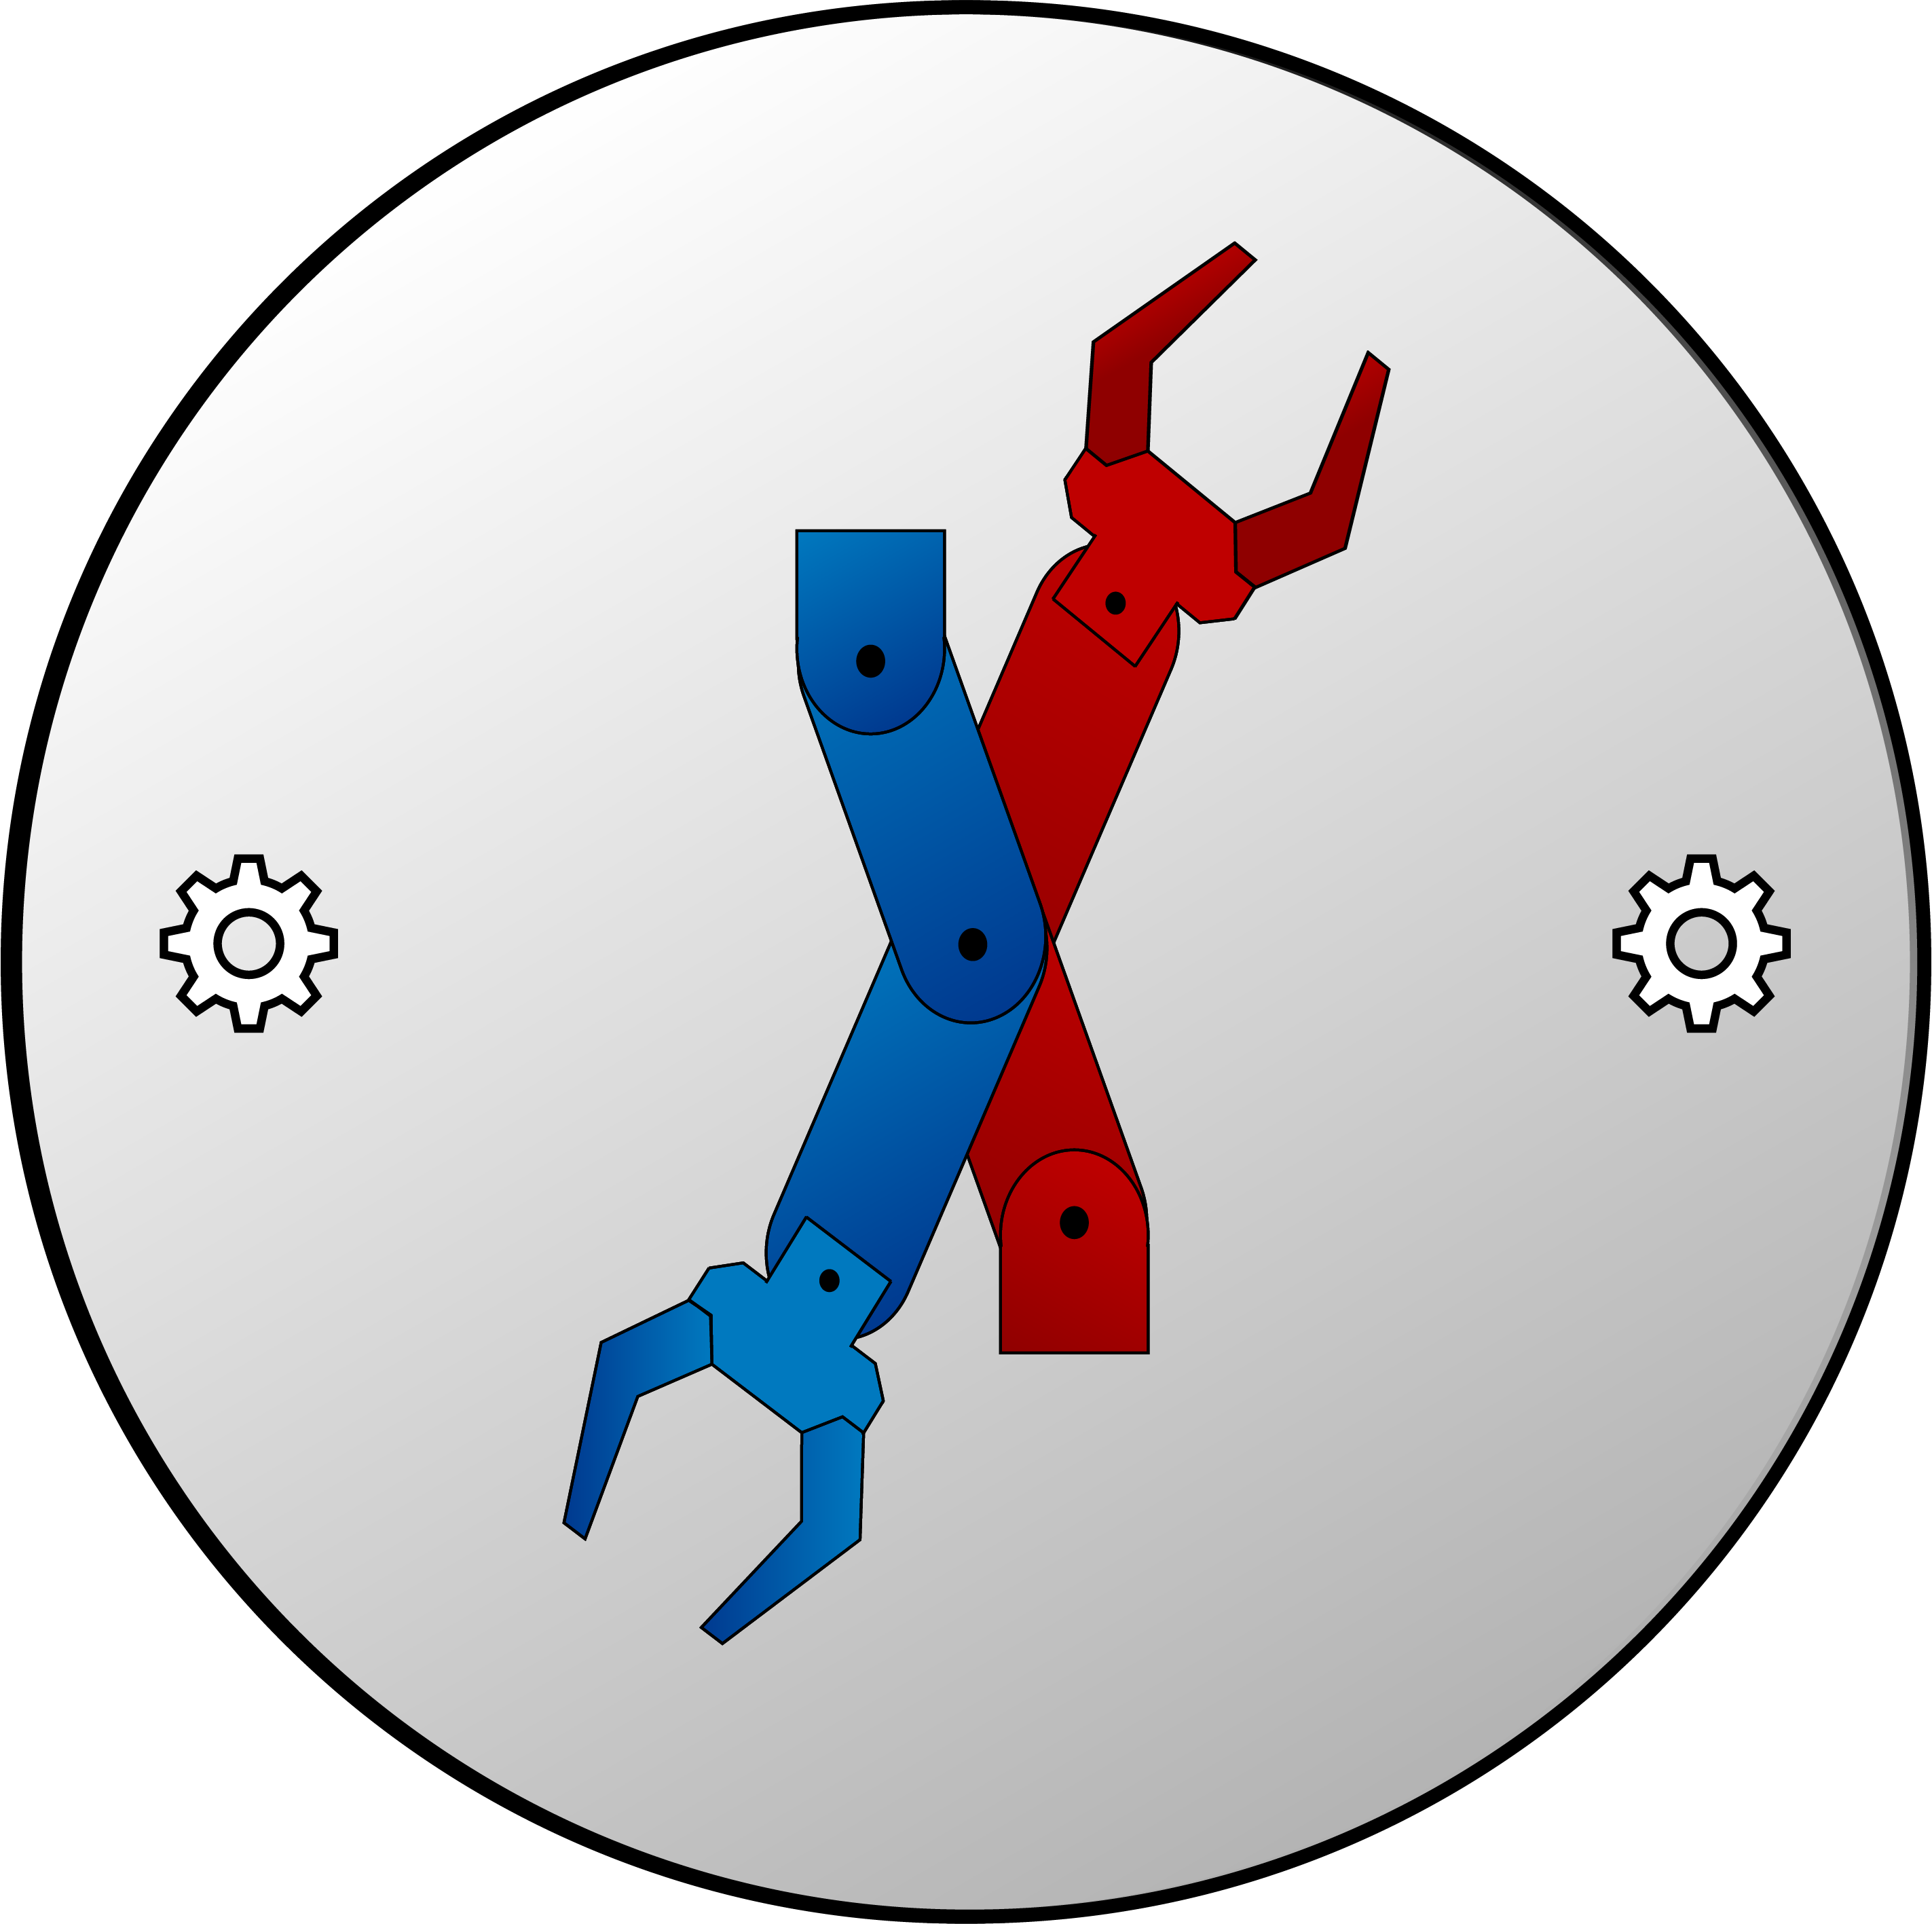
\includegraphics[width=.45\textwidth]{logo}
\vfill
\flushleft
ME 407 \\
Preliminary Design of Robotic Systems \\
Embry-Riddle Aeronautical University \\
\vspace{2ex}
\begin{minipage}[c]{.5\textwidth}
\flushleft

\includegraphics[width=.95\textwidth]{erau}
\end{minipage}%
\begin{minipage}[c]{.5\textwidth}
\flushright

\includegraphics[width=.8\textwidth]{text}
\end{minipage}
\end{titlepage}

\pagenumbering{roman}
% \begin{abstract}
  % Wordy words
% \end{abstract}
{\tableofcontents\let\clearpage\relax\listoffigures}
% {\tableofcontents\let\clearpage\relax\listoffigures\let\clearpage\relax\listoftables}
\clearpage
\newpage

% \section*{List Of Acronyms and Abbreviations}

% \begin{tabular}{rl}
%   $G$~:&Center of gravity of the bar \\
%   $\ell_0$~:& Spring unstretched length  \\
% \end{tabular}
% \normalsize
% \flushleft
% \singlespacing
% \newpage
\pagenumbering{arabic}

\section{Introduction}
\raggedright
\begin{figure}[htp]
  \centering
  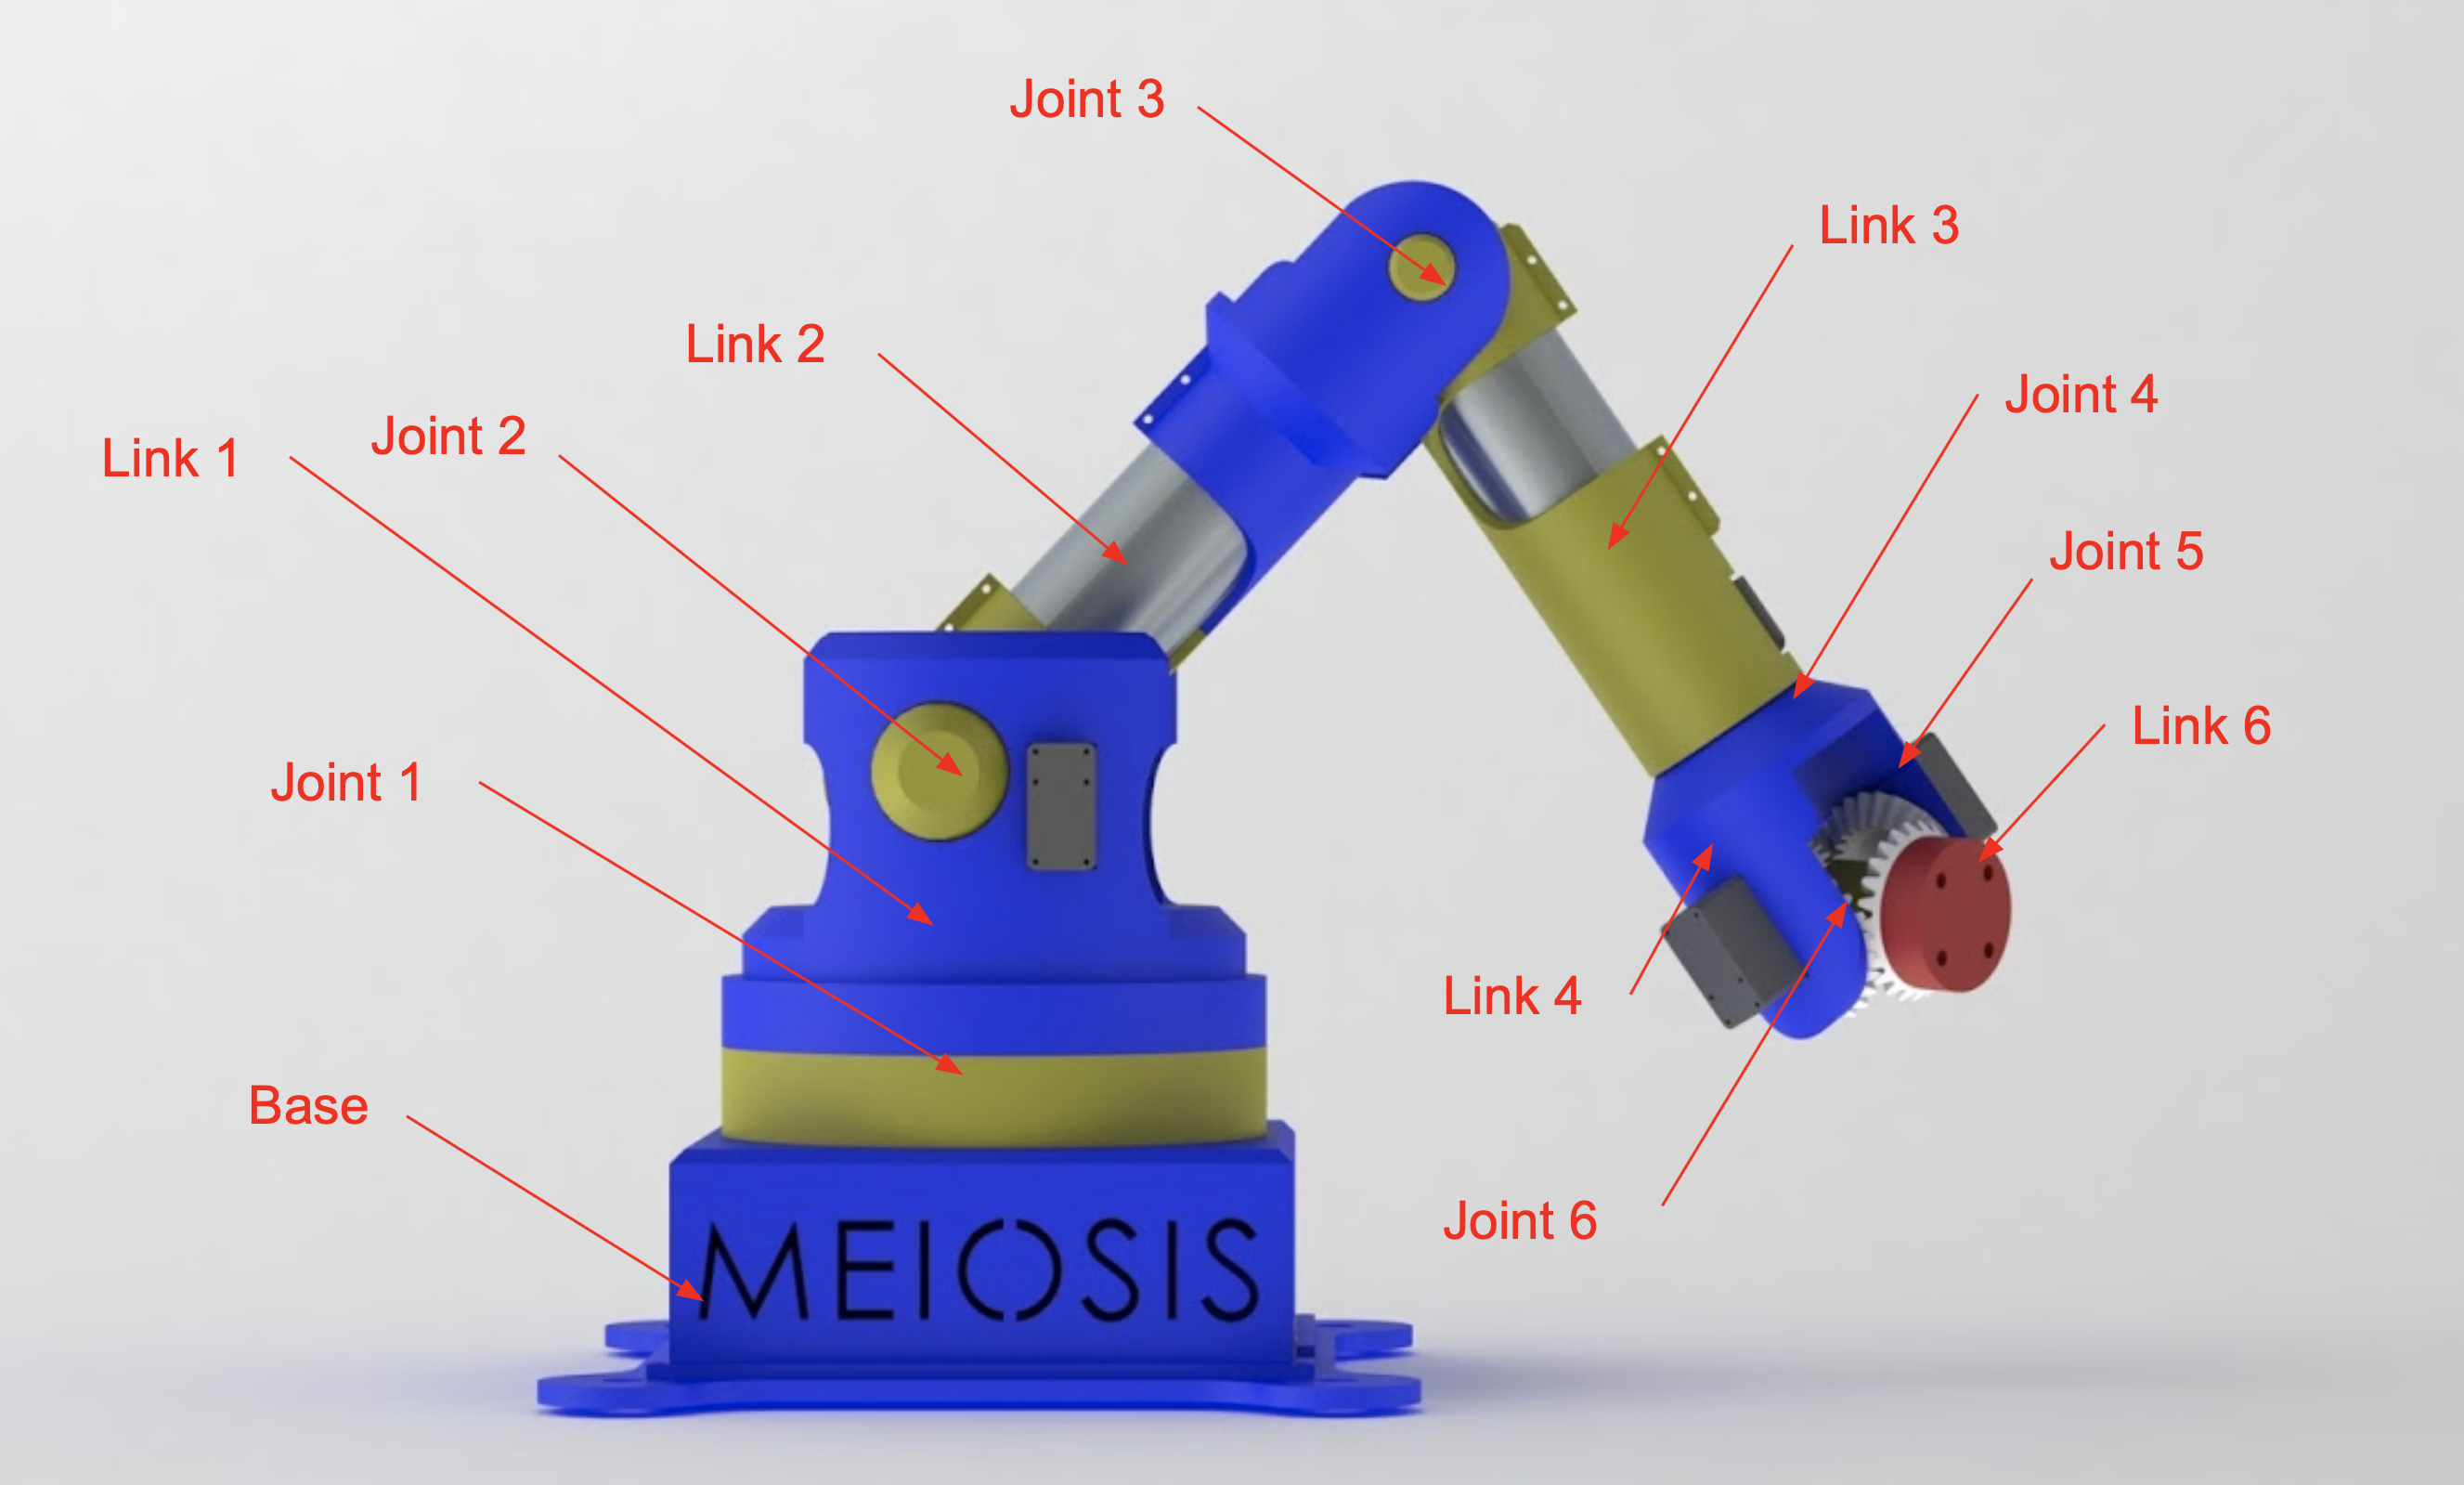
\includegraphics[frame,width=.75\textwidth]{model}
  \caption{Overview of Physical System}
  \label{fig:model}
\end{figure}
\section{Design Requirements}
\subsection{Hardware}

\subsubsection{The system shall cost the end-user no more than \$1000.}
\begin{enumerate}[label=\thesubsubsection.\alph*,leftmargin=3cm,font=\itshape]
  \item \textit{The cost for the MEIOSIS team to develop the manipulator shall cost no more than \$800.}
  \item \textit{The system shall cost the end-user no more than \$1000.}
\end{enumerate}

\subsubsection{The system shall be fully dexterous without being kinematically redundant.}
\begin{enumerate}[label=\thesubsubsection.\alph*,leftmargin=3cm,font=\itshape]
\item \textit{The system shall consist of six rotational joints connected by four links. The last three joints will create a spherical wrist.}
\end{enumerate}

\subsubsection{The system end effector shall maintain a positional accuracy magnitude of \(\pm 1\) mm and an orientation accuracy of \(\pm 5^{\circ}\) eigen angle from the base frame.}
To ensure that the robot has educational value, the accuracy must be defined so that any desired positions and movements are achieved.
\begin{enumerate}[label=\thesubsubsection.\alph*,leftmargin=3cm,font=\itshape]
  \item \textit{The system shall possess the ability to calibrate, or “zero,” the end effector position and orientation to within 1 degree of the manipulator’s precision. }
\end{enumerate}
\subsubsection{The system end effector shall maintain a pose repeatability magnitude between 0.1—1.5 mm for the position and \(\pm 4^{\circ}\) eigen angle from the base frame for the orientation.}
\begin{enumerate}[label=\thesubsubsection.\alph*,leftmargin=3cm,font=\itshape]
  \item \textit{Joint one and two of the system shall possess an angle error of no more than .025 degrees.}
  \item \textit{Joint three of the system shall possess an angle error of no more than .03 degrees.}
  \item \textit{Joints four, five, and six shall possess an angle error of no more than .29 degrees.}
\end{enumerate}
\subsubsection{The system’s reachable workspace shall be a hemisphere with a radius of 300-700 mm.}
This workspace will provide enough movement to manipulate objects in order to perform basic tasks.
\begin{enumerate}[label=\thesubsubsection.\alph*,leftmargin=3cm,font=\itshape]
  \item \textit{The length of link one, two, three, and the wrist shall be 220.8 mm, 250 mm, 200 mm, and 52.5 mm respectively.}
\end{enumerate}
\newpage
\subsubsection{The system’s dexterous workspace shall be a hemispherical shell within the reachable workspace with a thickness of 280 mm.}
This workspace will provide enough movement to manipulate objects in order to perform basic tasks. 280mm is slightly greater than the length of letter paper.
\begin{figure}[htp]
  \centering
  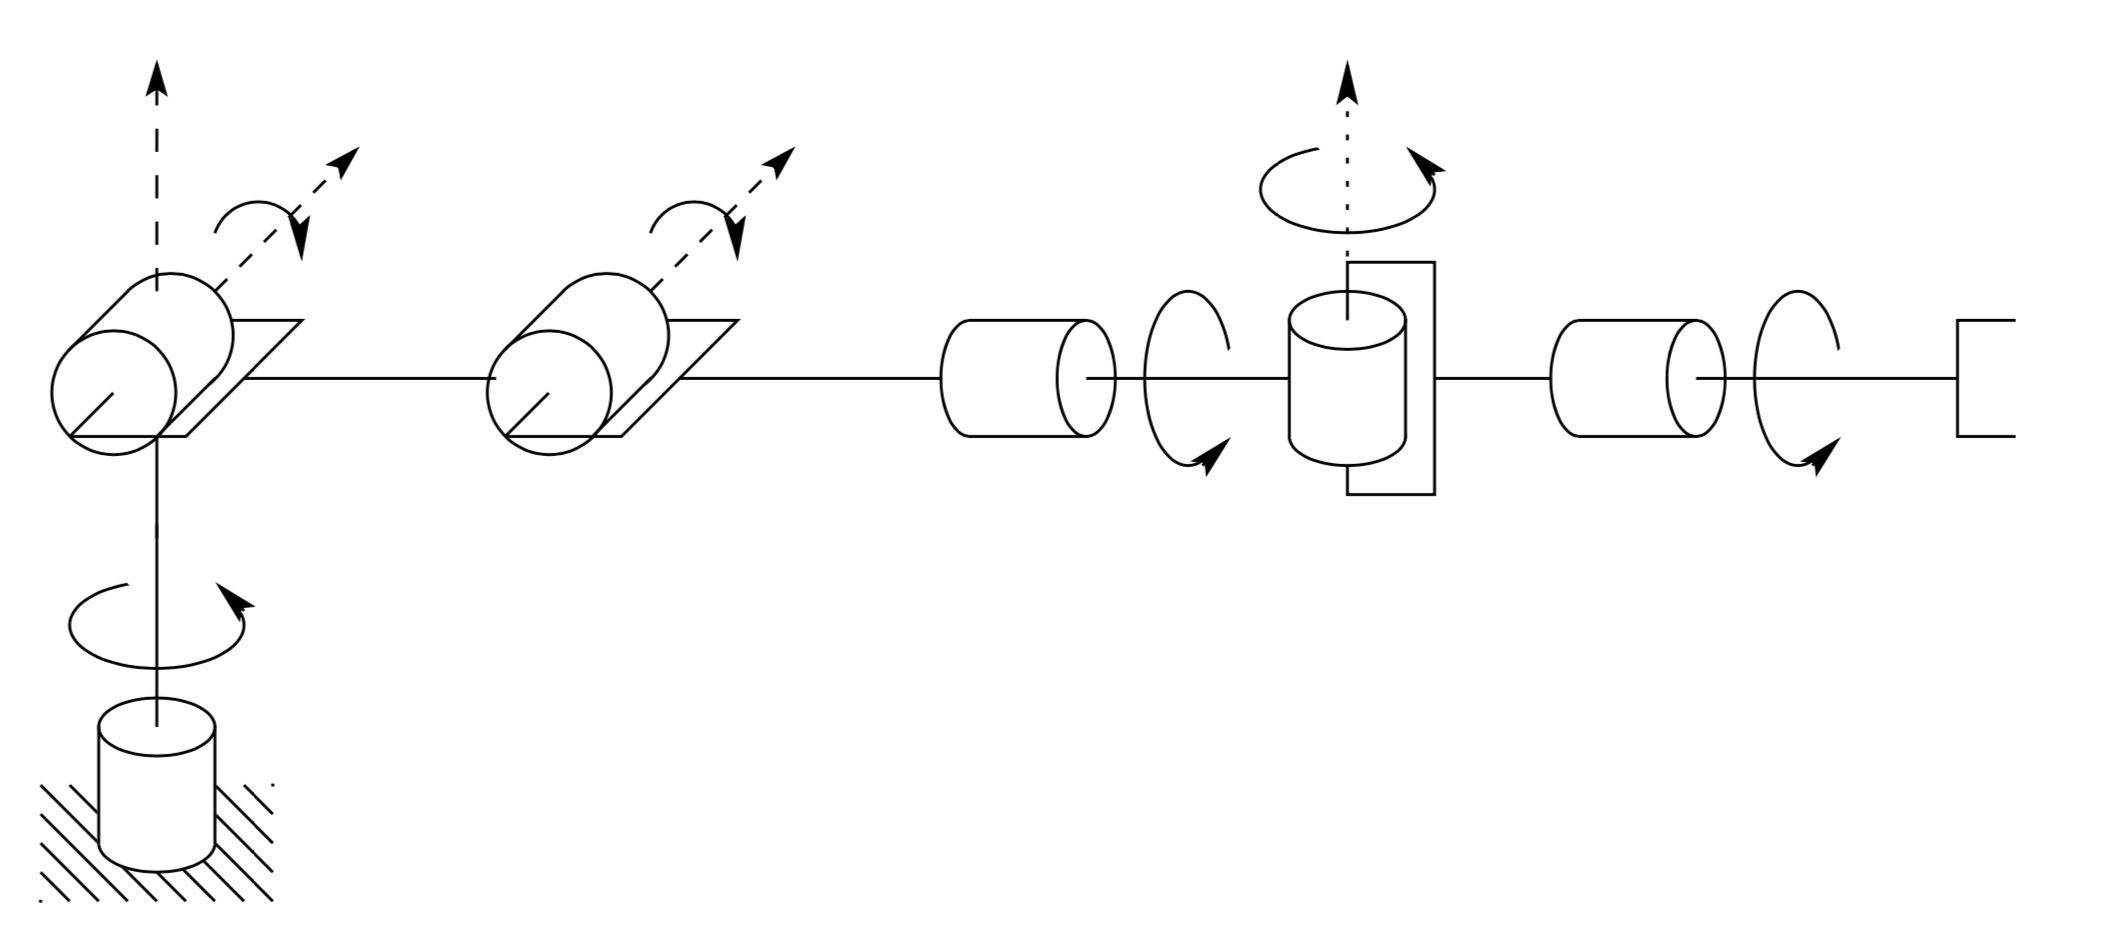
\includegraphics[width=.75\textwidth]{zero}
  \caption{Kinematic Model Representing Zeroed Configuration}
  \label{fig:zero}
\end{figure}
\begin{enumerate}[label=\thesubsubsection.\alph*,leftmargin=3cm,font=\itshape]
  \item \textit{With respect to the kinematic model shown above in Figure \ref{fig:zero}, the rotational limit of joint one, two, three, four, five, and six shall be \(\pm180^{\circ}\), \(\pm9.7^{\circ}\) to \(177.5^{\circ}\), \(-150.6^{\circ}\) to \(-19.3^{\circ}\), \(\pm180^{\circ}\), \(-180^{\circ}\) to \(-1.6^{\circ}\), and \(\pm180^{\circ}\).}
\end{enumerate}
\subsubsection{The system shall have a removable end effector capable of picking and placing a low-odor chisel tip Expo dry erase marker.}
This creates a robot capable of performing a variety of basic tasks, which enhances its educational value.
\begin{enumerate}[label=\thesubsubsection.\alph*,leftmargin=3cm,font=\itshape]
  \item \textit{The system will use an actuatable parallel gripper that can close to 18mm.}
  \item \textit{The end effector will attach to the manipulator using screws configured in a pattern that can mount a Dynamixel AX-12A servo.}
\end{enumerate}

\subsubsection{The system shall be able to write with a low-odor chisel tip Expo dry erase marker.}
\begin{enumerate}[label=\thesubsubsection.\alph*,leftmargin=3cm,font=\itshape]
  \item \textit{The end effector shall be capable of applying a gripping force of 0.028449 Newtons as to prevent slipping while writing.}
\end{enumerate}

\subsection{Software}
\subsubsection{The system shall be open source.}
This will create an easily obtainable, low cost method of distributing the system’s source code, which may be modified for personal use.
\begin{enumerate}[label=\thesubsubsection.\alph*,leftmargin=3cm,font=\itshape]
  \item \textit{The software shall be hosted publicly on an online repository and maintain an MIT license for distribution.}
\end{enumerate}
\subsubsection{The system shall be capable of operating given only desired end effector cartesian coordinates specified with respect to the base frame.}
\begin{enumerate}[label=\thesubsubsection.\alph*,leftmargin=3cm,font=\itshape]
  \item \textit{The system shall have a user interface capable of accepting user input.}
  \item \textit{The system shall be capable of performing floating point arithmetic for the inverse kinematic calculations.}
\end{enumerate}
\end{document}
